% Kopfzeile beim Kapitelanfang:
\fancypagestyle{plain}{
%Kopfzeile links bzw. innen
\fancyhead[L]{\Large Vorlesung 19 (16.12.2013)}
%Kopfzeile rechts bzw. außen
\fancyhead[R]{}}
%Kopfzeile links bzw. innen
\fancyhead[L]{\Large Vorlesung 19 (16.12.2013)}
%Kopfzeile rechts bzw. außen
\fancyhead[R]{}
% **************************************************
\phantomsection
\addcontentsline{toc}{section}{Der natürliche Logarithmus (logarithmus naturalis)}
\section*{Der natürliche Logarithmus (logarithmus naturalis)}
\section{Lemma}\label{10.5}
$exp: \R \to (0,\infty), x \mto e^x$ ist stetig, streng monoton wachsend und bijektiv.\nl
\begin{tikzpicture}
\draw[->] (-2,0)--(2,0);
\draw[->] (0,-0.5)--(0,2);
\draw[color=blue,domain=-2:0.6931471] plot (\x, {exp(\x)});
\draw (0,1) node {$\bullet$} node[left] {$1$};
\end{tikzpicture}

\subsection*{Beweis}
Stetigkeit, Satz \ref{9.5}, Strenge Monotonie\nl
Sei $x \in \R, h > 0 \Ra e^{x+h} - e^x = \underbrace{e^x}_{>0} (e^h-1) = e^x \underbrace{\sum_{k=1}^\infty \frac{h^k}{k!}}_{>0} > 0$\\
$\Ra exp$ ist injektiv.\\
$\lim_{x \to +\infty} e^x = +\infty, \lim_{x \to -\infty} e^x = 0$\\
$exp$ stetig $\underset{\text{ZWS}}{\Ra} exp$ nimmt jeden Wert aus $(0,\infty)$ an $\Ra exp$ ist surjektiv.

\subsection*{Konsequenz}
$exp: \R \to (0,\infty)$ hat eine Umkehrfunktion $ln: (0,\infty) \to \R$, den \underline{natürlichen Logarithmus} (logarithmus naturalis).\\
$ln$ ist streng monoton wachsend, stetig und bijektiv.\nl
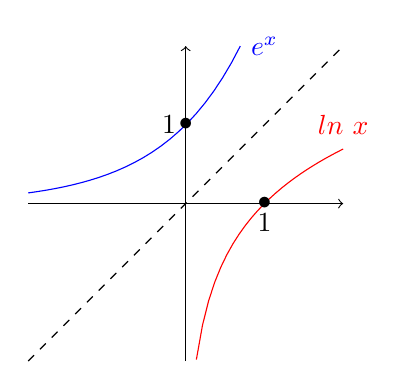
\begin{tikzpicture}
\draw[->] (-2,0)--(2,0);
\draw[->] (0,-2)--(0,2);
\draw[color=blue,domain=-2:0.6931471] plot (\x, {exp(\x)});
\draw[color=red,domain=0.13534:2] plot (\x, {ln(\x)});
\draw[dashed] (-2,-2)--(2,2);
\draw[color=blue] (1,2) node {$e^x$};
\draw[color=red] (2,1) node {$ln \ x$};
\draw (0,1) node {$\bullet$} node[left] {$1$};
\draw (1,0) node {$\bullet$} node[below] {$1$};
\end{tikzpicture}

\subsubsection*{Spezielle Werte}
$ln \ 1 = 0$\\
$ln \ e = 1$\\
$\lim_{x \downarrow 0} ln \ x = -\infty$, $\lim_{x \to +\infty} ln \ x = +\infty$ (aus Graphen ablesen)

\newpage

\section{Satz}\label{10.6}
\en{
\item $x,y > 0 \Ra$ \fbox{$ln(xy) = ln \ x + ln \ y$} \underline{Funktionalgleichung}
\item $ln\left(\frac{1}{x}\right) = -ln \ x$
\item $\lim_{x \to 0} \frac{ln(1+x)}{x} = 1$
}

\subsection*{Beweis}
\en{
\item $e^{ln(xy)} = xy = e^{ln \ x} \cdot e^{ln \ y} = e^{ln \ x + ln \ y} \underset{exp \text{ bij.}}{\Ra} ln(xy) = ln \ x + ln \ y$
\item $ln\left(x \cdot \frac{1}{x}\right) = ln \ 1 = 0$, anderersetis: $ln\left(x \cdot \frac{1}{x}\right) \underset{\text{(1)}}{=} ln \ x + ln\left(\frac{1}{x}\right)$
\item $y := ln(1+x) \Lra x=e^y-1, x \to 0 \Lra y \to 0$\\
$\lim_{x \to 0} \frac{ln(1+x)}{x} = \lim_{y \to 0} \frac{y}{e^y-1} = 1$ (\ref{9.14}, 4)
} \qed

\phantomsection
\addcontentsline{toc}{section}{Exponentialfunktion zu allgemeinen Basen}
\section*{Exponentialfunktion zu allgemeinen Basen}
Sei $a \in \R, a > 0$. Ziel: Definition von $a^x, x \in \R$.\\
$x = \frac{p}{q}, p \in \Z, q \in \N \Ra a^{p}{q} := \sqrt[q]{a^p} = \sqrt[q]{(e^{ln \ a})^p} \underset{\text{FG}}{=} \sqrt[q]{e^{p \ ln \ a}} = e^{\frac{p}{q} ln \ a}$

\section{Definition: Exponentialfunktion zu allgemeinen Basen}\label{10.7}
\fbox{$exp_a (x) = a^x := e^{x \ ln \ a}$} ($x \in \R$) ist die \underline{Exponentialfunktion zur Basis $a > 0$}.

\section{Eigenschaften}\label{10.8}
\en{
\item $a^0 = 1$; $q \in \N \Ra \sqrt[q]{a} = a^{\frac{1}{q}}$
\item $a^{x+y} = a^x \cdot a^y$; \fbox{$a^{-x} = \frac{1}{a^x}$}\\
Denn: $a^{x+y} = e^{(x+y) ln \ a} = e^{x \ ln \ a} \cdot e^{y \ ln \ a} = a^x \cdot a^y$
\item $a,b > 0 \Ra a^x b^x = (ab)^x$; $(a^x)^y = a^{xy}$ (Übung)
\item $exp_a: \R \to (0,\infty)$ bijektiv und stetig (Kompos. stetige Funktion)
\item $a > 1 \underset{ln \ a > 0}{\Ra} exp_a$ s.m.w. auf $\R$\\
$a < 1 \underset{ln \ a < 0}{\Ra} exp_a$ s.m.f. auf $\R$
}
Konsequenz aus (4) und (5): $exp_a: \R \to (0,\infty)$; $a \neq 1$ ($exp_1 \equiv 1$) hat eine Umkehrfunktion $log_a: (0,\infty) \to \R$, den \underline{Logarithmus zur Basis $a$}, streng monoton wachsend (falls $a>1$) bzw. fallend (falls $a<1$), stetig und bijektiv\nl
Insbes.: $exp_e = exp$, $log_e = ln$\\
Wichtig in der Informatik: $a=1, log_2$

\phantomsection
\addcontentsline{toc}{section}{Potenzfunktionen}
\section*{Potenzfunktionen}\label{Potenzfunktionen}
Fixiere Exponenten $s \in \R$.\\
\fbox{$p_s(x) := x^s = e^{s \ ln \ x}$, $x \in (0,\infty)$} ist die \underline{Potenzfunktion zum Exponenten $s$}.\\
Speziell: $p_{1/2}(x) = \sqrt{x}$, $p_{-1}(x) = \frac{1}{x}$\\
$p_s$ ist stetig auf $(0,\infty)$ (Kompos. stetiger Funktion)\nl
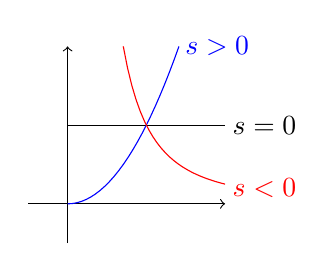
\begin{tikzpicture}
\draw[->] (-0.5,0)--(2,0);
\draw[->] (0,-0.5)--(0,2);
\draw[domain=0:2] plot (\x, {1});
\draw(2.5,1) node {$s=0$};
\draw[color=blue,domain=0:1.4142136] plot (\x, {\x^2});
\draw[color=blue] (1.9,2) node {$s>0$};
\draw[color=red,domain=0.707106:2] plot (\x, {1/(\x^2)});
\draw[color=red] (2.5,0.2) node {$s<0$};
\end{tikzpicture}\nl
Sei $s > 0 \Ra \lim_{x \downarrow 0} p_s(x) = \lim_{x \downarrow 0} e^{s \ ln \ x} = 0$\\
$\Ra p_s$ ist stetig fortsetzbar in $0$ mit $p_s(0)=0$

\chapter{Differentialrechnung}\label{P11}
\section{Definition: Die Ableitung}\label{11.1}
Sei $D \subseteq \R, f: D \to \R$ eine Funktion.\\
$f$ heißt \underline{differenzierbar} in $x_0 \in D$, falls $f'(x_0) := \lim_{\underset{(x \neq x_0)}{x \to x_0}} \underbrace{\frac{f(x)-f(x_0)}{x-x_0}}_{\text{Differenzenquotient in } x_0} \in \R$ existiert.

\subsection*{Bezeichnung}
$f$ ist differenzierbar auf $D :\Lra f$ ist differenzierbar in allen $x_0 \in D$\\
$f'(x_0)$: \underline{Ableitung} von $f$ im Punkt $x_0$

\subsection*{Geometrische Deutung}
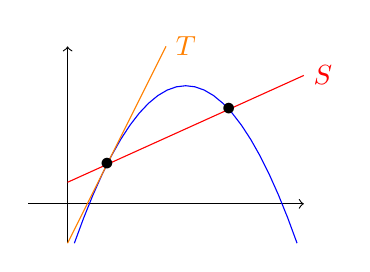
\begin{tikzpicture}
\draw[->] (-0.5,0)--(3,0);
\draw[->] (0,-0.5)--(0,2);
\draw[color=blue,domain=0.0857864:2.91421] plot (\x, {-(\x-1.5)^2+1.5});
\draw[color=red] (0,0.273861)--(3,1.63069557) node[right] {$S$};
\draw[color=orange] (0,-0.5)--(1.25,2) node[right] {$T$};
\draw (0.5,0.5) node {$\bullet$};
\draw (2.04772,1.2) node {$\bullet$};
\end{tikzpicture}\\
\emph{Bez.: \textbf{S}ekante, \textbf{T}angente}

\subsection*{Gleichung der Geraden durch $p_0$ und $p$}
$S(t) = f(x_0) + \underbrace{\frac{f(x)-f(x_0)}{x-x_0}}_{\text{Steigung}} \cdot (t-x_0)$, $t \in \R$\\
Falls $f'(x_0)$ existiert, so geht mit $x \to x_0$ die Sekante in die Tangente an dem Graphen $\Gamma_f$ im Punkt $p_0$ über; deren Gleichung ist:\\
$T(t)=f(x_0)+f'(x_0) \cdot (t-x_0)$, $t \in \R$

\newpage

\section{Beispiele}\label{11.2}
\en{
\item $f: \R \to \R, f(x) = c$ (konst. Funktion) mit $c \in \R$\nl
\begin{tikzpicture}
\draw[->] (-0.5,0)--(2,0);
\draw[->] (0,-0.5)--(0,2);
\draw[color=blue,domain=-0.5:2] plot (\x, {1});
\draw (-0.3,1.3) node {$c$};
\end{tikzpicture}\nl
$f(x)-f(x_0) = 0 \forall x \Ra f$ differenzierbar auf $\R$ mit $f' \equiv 0$ (identisch $0$)
\item $f(x)=x^n$, $n \in \N$, $x_0 \in \R$\\
$\frac{x^n-x_0^n}{x-x_0} = x^{n-1} + x_0 x^{n-2} + \ldots + x_0^{n-1} x + x_0^{n-1} \underset{x \to x_0}{\to} n x_0^{n-1}$\\
$f$ differenzierbar auf $\R$, $f'(x) = \frac{d}{dx}(x^n) = n x^{n-1}$\nl
\underline{Bemerkung}: Bezeichnung: $f'(x_0) = \frac{d}{dx} f(x_0)$
\item $f(x) = e^{ax}$ mit $a \in \R \Ra f$ differenzierbar auf $\R$ mit \fbox{$\frac{d}{dx}(e^{ax}) = a \cdot e^{ax}$}\nl
Insbes.: $exp' = exp$ ($a=1$)\\
Denn: Sei $a \neq 0$. $\frac{e^{ax}-e^{ax_0}}{x-x_0} \underset{h := x-x_0}{=} \frac{e^{a(x_0+h)}-e^{ax_0}}{h}$\\
$\underset{\text{FG}}{=} a \cdot e^{ax_0} \cdot \underbrace{\frac{e^{ah} - 1}{ah}}_{\to 1 \text{ für } h \to 0} \underset{h \to 0}{\to} a \cdot e^{ax_0}$\\
Formel gilt auch, falls $a=0$: $\frac{d}{dx}(1)=0$
\item \fbox{$ln'(x)=\frac{1}{x}$} ($x>0$)\nl
Denn: $x>0, h \neq 0 \Ra \frac{ln(x+h)-ln \ x}{h} \underset{\text{FG von }ln}{=} \frac{ln\left(\frac{x+h}{x}\right)}{h} = \underbrace{\frac{ln\left(1+\frac{h}{x}\right)}{\frac{h}{x}}}_{\to 1 \text{ für } h \to 0 \text{ (\ref{10.6})}} \cdot \frac{1}{x}$
\item \fbox{$\begin{array}{l} sin'(x) = cos(x) \\ cos'(x)=-sin(x) \end{array}$} ($x \in \R$)\nl
\underline{Beweis für sin} (cos analog): $h \neq 0, x \in \R \Ra$\\
$\frac{sin(x+h)-sin(x)}{h} \underset{\text{Add.Thm.}}{=} \frac{sin(x) \cdot cos(h) + cos(x) \cdot sin(h) - sin(x)}{h}$\\
$= sin(x) \cdot \underbrace{\frac{cos(h)-1}{h}}_{\text{(*) } \to 0 \text{ für } h \to 0} + cos(x) + \underbrace{\frac{sin(h)}{h}}_{\to 1 \text{ für } h \to 0}$\\
Zu (*): $\frac{cos(h)-1}{h} = h \cdot \underbrace{\frac{cos(h)-1}{h^2}}_{\to \frac{1}{2} \text{ für } h \to 0 \text{ Übg.}} \to 0$ \qed
}